\section{Coordinate System}
\label{chapter:design:coordinatesystem}

	The Cartesian \termdef{Coordinate System} of the 3-dimensional space of a scene has two properties that need to be defined in order to position objects therein:

	\begin{smalllist}
		\item Handedness: The direction the third vector points to, when the first two are defined.
		\item Orientation: The directions the three vectors point to.
	\end{smalllist}

	The orientation is unnecessary for the definition of the coordinate system from a mathematical point of view, since all orientations with the same handedness can be transformed to each other using a single rotation around the origin according to Euler's rotation theorem\cite{PP07}. But since human orientation rather happens in terms of relative directions - up, down, left, right, forward, backward - those directions are mapped to absolute vectors within the coordinate system.

	The lack of a standard mapping\footnote{OpenGL and Direct3D9 both use X/Y for left/up but differ in handedness, OpenGL defining negative Z as the forward vector\cite{Buss:2003:CGM:861813}, whereas Direct3D9 chooses positive Z\cite{jones2004beginning}. Panda3d, on the other hand, implements a right-handed coordinate system where X, Y and Z correspond to right, forward and upward\cite{Goslin:2004:PGE:1032275.1032359}.} is taken as an indicator that it is best left to personal preference. Although changing the coordinate system after having used it for positioning might lead to unexpected results, it is still possible to set the desired coordinate system at run-time.

	Formally, the desired orientation serves but a single purpose: to assign a default rotation to newly created objects. All rotatable objects have a predefined orientation, or predefined directions that are considered that object's forward, right and up vectors. The orientation of the coordinate system rotates all new objects to align those directional vectors to those of the coordinate system's orientation. Figure \ref{fig:RotatedSpotLight} shows a newly created spot light that was positioned facing forward in the coordinate system orientation of Direct3D9 - assuming that the forward orientation of a spot light is defined by the direction vector its light is emitted to.

	\begin{figure}[htbp]
		\centering
		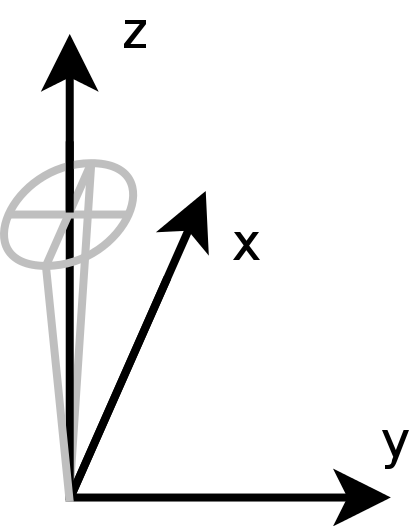
\includegraphics[width=4cm]{images/rotatedspotlight.png}
		\caption{A spot light facing ``forward'' in the Direct3D9 coordinate system, assuming its front-side is the direction the light is emitted to.}
		\label{fig:RotatedSpotLight}
	\end{figure}

	Although relative axes are defined in many engines, they are not an integral part of the API. The orientation is still used as a default alignment of new objects - an untransformed object is left of an untransformed camera - but a ``rotation to the left'' does not exist in any of the reference APIs, rendering the original definition less useful than it could be. Whatever the orientation of the coordinate system is, one must fall back to the usage of the named coordinate axes $X$, $Y$ and $Z$.

	We will introduce relative orientation into the API to make stronger use of the already-present orientation capabilities of humans in the real world. If the Direct3D9 alignment of the coordinate system was chosen, a rotation around the $Y$ axis can be expressed as a rotation to the right: \inlinecode{rotateRight(Degree(90));} We will see in the next Section that the design of such a simplistic system has a drawback: the reference point for rotations is very ambiguous.

